%        File: arfc-beamer.tex
%     Created: Sun May 5 10:00 PM 2013 C
%


%\documentclass[11pt,handout]{beamer}
\documentclass[9pt]{beamer}
\usetheme[white]{Illinois}
%\title[short title]{long title}
\title[Short Title]{$S_N$ Method for Neutron Transport}
%\subtitle[short subtitle]{long subtitle}
\subtitle[Short SubTitle]{Applied to the Ackroyd-Riyait Benchmark}
%\author[short name]{long name}
\author[Your Name]{Elijah Capps, Liam Pohlmann
\\Advanced Reactors and Fuel Cycles Group}
%\date[short date]{long date}
\date[03.31.2026]{March 31, 2026}
%\institution[short name]{long name}
\institute[UIUC]{University of Illinois at Urbana-Champaign}

%\usepackage{bbding}
\usepackage{amsfonts}
\usepackage{amsmath}
\usepackage{bm}
\usepackage{xspace}
\usepackage{graphicx}
\usepackage{subcaption}
\usepackage{booktabs} % nice rules for tables
\usepackage{microtype} % if using PDF
\usepackage{bigints}
% \usepackage{minted2}
\usepackage{physics}
\usepackage[noabbrev,capitalize]{cleveref}

% algorithms
\usepackage{algorithm}
\usepackage{algpseudocode}
\usepackage{algpseudocodex}

\usepackage{tikz}
\usetikzlibrary{positioning}
\usetikzlibrary{shapes.geometric, arrows}
\tikzstyle{startstop} = [rectangle, rounded corners, 
minimum width=3cm, 
minimum height=1cm,
text centered, 
draw=black, 
fill=red!30]

\tikzstyle{io} = [trapezium, 
trapezium stretches=true, % A later addition
trapezium left angle=70, 
trapezium right angle=110, 
minimum width=3cm, 
minimum height=1cm, text centered, 
draw=black, fill=blue!30]

\tikzstyle{process} = [rectangle, 
minimum width=3cm, 
minimum height=1cm, 
text centered, 
text width=3cm, 
draw=black, 
fill=orange!30]

\tikzstyle{decision} = [diamond, 
minimum width=3cm, 
minimum height=1cm, 
text centered, 
draw=black, 
fill=green!30]
\tikzstyle{arrow} = [thick,->,>=stealth]
\usepackage{xcolor}

\definecolor{SourceColor}{HTML}{fcfdbf}
\definecolor{VoidColor}{HTML}{180f3d}
\definecolor{MaterialColor}{HTML}{cd4071}

\newcommand{\ohat}{\hat{\Omega}}
\newcommand{\rvec}{\mathbf{r}}
\newcommand{\psifullprime}{\psi\left(\mathbf{r},\hat{\Omega}',E',t\right)}
\newcommand{\psifull}{\psi\left(\mathbf{r},\hat{\Omega},E,t\right)}
\newcommand{\psisimple}{\psi\left(\mathbf{r},\hat{\Omega}\right)} % "psi simple"
\newcommand{\psiplus}{\psi^+}
\newcommand{\intelems}{\int_{\mathcal{A}}\int_{\tau}}
\newcommand{\elemdifs}{\dd \tau \dd \ohat}
\newcommand{\sigt}{\Sigma_t}

\allowdisplaybreaks

\newcommand{\units}[1] {\:\text{#1}}%
\newcommand{\SN}{S$_N$}%{S$_\text{N}$}%{$S_N$}%
%Those icons in the references are terrible looking
\setbeamertemplate{bibliography item}[text]

%%%% Acronym support

\usepackage[acronym,toc]{glossaries}
\include{acros}

\makeglossaries

%try to get rid of header on title page\dots
\makeatletter
    \newenvironment{withoutheadline}{
        \setbeamertemplate{headline}[default]
        \def\beamer@entrycode{\vspace*{-\headheight}}
    }{}
\makeatother

\makeatother
\setbeamertemplate{footline}
{
  \leavevmode%
  \hbox{%
    \rightline{\insertframenumber{} / \inserttotalframenumber\hspace*{1ex}}
  }%
  \vskip0pt%
}
\makeatletter
% This will add figure numbers to captions.
\setbeamertemplate{caption}[numbered]

\begin{document}
%%%%%%%%%%%%%%%%%%%%%%%%%%%%%%%%%%%%%%%%%%%%%%%%%%%%%%%%%%%%%
%% From uw-beamer Here's a handy bit of code to place at
%% the beginning of your presentation (after \begin{document}):
\newcommand*{\alphabet}{ABCDEFGHIJKLMNOPQRSTUVWXYZabcdefghijklmnopqrstuvwxyz}
\newlength{\highlightheight}
\newlength{\highlightdepth}
\newlength{\highlightmargin}
\setlength{\highlightmargin}{2pt}
\settoheight{\highlightheight}{\alphabet}
\settodepth{\highlightdepth}{\alphabet}
\addtolength{\highlightheight}{\highlightmargin}
\addtolength{\highlightdepth}{\highlightmargin}
\addtolength{\highlightheight}{\highlightdepth}
\newcommand*{\Highlight}{\rlap{\textcolor{HighlightBackground}
    {\rule[-\highlightdepth]{\linewidth}{\highlightheight}}}}
%%%%%%%%%%%%%%%%%%%%%%%%%%%%%%%%%%%%%%%%%%%%%%%%%%%%%%%%%%%%%
%%--------------------------------%%
\begin{withoutheadline}
  \frame{
    \titlepage
  }
\end{withoutheadline}

%%--------------------------------%%
\AtBeginSection[]{
  \begin{frame}
    \frametitle{Outline}
    \tableofcontents[currentsection]
  \end{frame}
}

\section{Background and Motivation}
\subsection{Neutron Transport Equation}
\begin{frame}
        \frametitle{Neutron Transport Equation}
        The general linear \gls{bte} with an isotropic external source is~\cite{Larsen2010}:
        \begin{multline}\label{eq:general-bte}
                \frac{1}{v}\pdv{\psifull}{t} + \ohat\cdot \grad \psifull+\Sigma_t\left(\rvec,E\right)\psifull=\\= \int_{0}^{\infty}\int_{4\pi}\Sigma_s \left(\rvec,\ohat'\cdot \ohat,E'\rightarrow E\right)\psifullprime\dd \ohat' \dd E' +\\+ \frac{\chi \left(\rvec,E\right)}{4\pi }\int_{0}^\infty \int_{4\pi}\nu \Sigma_f \left(\rvec,E'\right)\psifullprime \dd \ohat ' \dd E' +\frac{Q\left(\rvec,E,t\right)}{4\pi}
        \end{multline}
        where $\psifull$ is the \textit{neutron angular flux}, $\ohat$ is the \textit{solid angle}, $E$ is the energy, $t$ is the time, $\rvec$ is the position vector, $\Sigma_s \left(\rvec,\ohat'\cdot \ohat,E'\rightarrow E\right)$ is the \textit{double-differential scattering cross section}, $\chi \left(\rvec,E\right)$ is the \textit{fission-born neutron energy spectrum}, $\nu$ is the \textit{average number of neutrons born per fission event}, $\Sigma_f$ is the \textit{macroscopic fission cross section}, and $Q\left(\rvec,E,t\right)$ is the \textit{independent isotropic neutron source}.
\end{frame}

\begin{frame}[allowframebreaks]
        \frametitle{Neutron Transport Equation}
        Each of the above terms has a physical significance and represent a conservation law.
        The losses are:
        \begin{subequations}
                \begin{equation}\label{eq:time-dep-term}
                        \frac{1}{v}\pdv{\psifull}{t} = \text{Time-dependence of angular flux}
                \end{equation}
                \begin{equation}\label{eq:streaming-term}
                        \ohat\cdot \grad \psifull = \text{Neutron loss to streaming}
                \end{equation}
                \begin{multline}\label{eq:interaction-term}
                        \Sigma_t\left(\rvec,E\right)\psifull \\= \text{Neutron losses to interactions with surroundings}
                \end{multline}
                \framebreak

                The sources are:
                \begin{multline} \label{eq:inscattering-term}
                        \int_{0}^{\infty}\int_{4\pi}\Sigma_s \left(\rvec,\ohat'\cdot \ohat,E'\rightarrow E\right)\psifullprime\dd \ohat' \dd E' \\= \text{Inscatter source}
                \end{multline}
                \begin{equation} \label{eq:fission-term}
                        \frac{\chi \left(\rvec,E\right)}{4\pi }\int_{0}^\infty \int_{4\pi}\nu \Sigma_f \left(\rvec,E'\right)\psifullprime \dd \ohat ' \dd E' = \text{Fission source}
                \end{equation}
                \begin{equation} \label{eq:indep-source-term}
                        \frac{Q\left(\rvec,E,t\right)}{4\pi} = \text{Independent volumetric, isotropic source}
                \end{equation}
        \end{subequations}
\end{frame}



\subsection{Problem Description}
\input{ar_problems.tex}

\subsection{Simplification of the Transport Equation}
\input{bte_simplification.tex}

\subsection{Even and Odd Parity Equations}
\input{even-odd-parity.tex}

\section{Finite Angular Elements - Methods}

\subsection{Finite Element Method}
\begin{frame}
  \frametitle{Weak Form}
  Note the following vector calculus identity for a scalar function $\psi$ and vector $\vec{A}$:
  \begin{equation}
    \label{eq:vec-calc-identity}
    \div \left(\psi\vec{A}\right)=\psi\div\vec{A}+\vec{A}\cdot\grad\psi
  \end{equation}
  Let $v=v(x,y,\theta,\varphi)$ be a test function.
  Multiplying \cref{eq:even-parity-equation} by $v$, integrating over an angular and spatial element gives, and applying \cref{eq:vec-calc-identity} twice gives the weak form:
  \begin{multline}\label{eq:general-weak-form}
    -\frac{1}{\sigt}\int_{\mathcal{A}}\oint_{\partial \tau}v\left(\ohat\cdot\grad{\psiplus}\right)\ohat\cdot\hat{n}\dd s\dd\ohat+\frac{1}{\sigt}\intelems\left(\ohat\cdot\grad{\psiplus}\right)\left(\ohat\cdot\grad{v}\right)\elemdifs+\\+
    \intelems v\sigt \psiplus\elemdifs=\intelems vS\elemdifs
  \end{multline}
  where $\int_\tau$ is the integral over a triangular spatial element, $\int_\mathcal{A}$ is the integral over an angular element, and $\hat{n}$ is the unit normal vector on in the spatial domain.
\end{frame}

\begin{frame}
  \frametitle{Boundary Conditions}
  Per Lewis \& Miller~\cite{lewisComputationalMethodsNeutron1993}, the vacuum boundary conditions are:
  \begin{equation}\label{eq:vacuum-bc}
    \ohat\cdot\grad{\psiplus}\pm\sigt\psiplus=0,\quad x,y\in \partial\Gamma_v,\ohat\cdot\hat{n}\lessgtr 0
  \end{equation}
  while the reflective boundary conditions are:
  \begin{equation}\label{eq:reflect-bc}
    \psiplus\left(\ohat\right)=\psiplus\left(\ohat '\right)
  \end{equation}
  \Cref{eq:reflect-bc} is trivially satisfied by the weak form, so it will not need further discussion.
  Inserting \cref{eq:vacuum-bc} into \cref{eq:general-weak-form}'s boundary condition gives:
  \begin{equation}
    -\frac{1}{\sigt}\int_{\mathcal{A}}\oint_{\partial \tau}v\left(\ohat\cdot\grad{\psiplus}\right)\ohat\cdot\hat{n}\dd s\dd\ohat=\pm \int_\mathcal{A}\oint_{\partial\tau_v}v\psiplus\left(\ohat\cdot\hat{n}\right)\dd s\dd \ohat
  \end{equation}
  Notice that the sign in the boundary term is guaranteed to be positive.

\end{frame}

\begin{frame}
  \frametitle{Weak Form}
  Noting the following definitions for $\theta\in[0,\pi]$, $\varphi\in[0,\pi/2]$:
  \begin{equation}
    \ohat\cdot\grad{\psiplus}=\mu\pdv{\psiplus}{x}+\eta\pdv{\psiplus}{y}+\xi\pdv{\psiplus}{z}
  \end{equation}
  \begin{equation}
    \ohat=\left(\underbrace{\cos\varphi}_\mu,\underbrace{\cos\theta\sin\varphi}_\eta,\underbrace{\sin\theta\sin\varphi}_\xi\right)
  \end{equation}
  and disregarding the $z-$ component (for 2D), we finally arrive at:
  \begin{multline}\label{eq:weak-form}
    \pm\int_{\mathcal{A}}\oint_{\partial\tau}v\psiplus\left(\mu n_x+\eta n_y\right)\dd s\dd\ohat +\\+\frac{1}{\sigt}
    \intelems\left(\mu\pdv{\psiplus}{x}+\eta\pdv{\psiplus}{y}\right)\left(\mu\pdv{v}{x}+\eta\pdv{v}{y}\right)\elemdifs+\\
    +\sigt\intelems v \psiplus\elemdifs=\intelems vS\elemdifs
  \end{multline}
\end{frame}

\begin{frame}
  \frametitle{Function Approximation}
  Let
  \begin{equation}
    \label{eq:function-approx}
    \psiplus \left(x,y,\theta,\varphi\right)\approx\sum_i\sum_j \psi_{ij}T_i(x,y)A_j(\theta,\varphi)
  \end{equation}
  for $i\in[1,n_t]$ for $n_t$ triangles in space, $j\in[1,n_a]$ for $n_a$ elements in solid angle.
  Inserting \cref{eq:function-approx} into \cref{eq:weak-form} and combining summations gives:
  \begin{multline}\label{eq:function-exp-fem}
    \pm\int_{\mathcal{A}}\oint_{\partial\tau}v\sum_{i,j} \psi_{ij}T_iA_j\left(\mu n_x+\eta n_y\right)\dd s\dd\ohat +\\+
    \frac{1}{\sigt}\intelems \left(\sum_{i,j}\left(\mu\pdv{T_i}{x}+\eta\pdv{T_i}{y}\right)A_j\psi_{ij}\right)\left(\mu\pdv{v}{x}+\eta\pdv{v}{y}\right)\elemdifs+\\+
    \sigt\intelems v\sum_{i,j} T_i A_j \psi_{ij}\elemdifs = \intelems vS\elemdifs
  \end{multline}
\end{frame}

\begin{frame}
  \frametitle{Galerkin Method}
  For the test function, we choose the same basis functions as in \cref{eq:function-approx}:
  \begin{equation}\label{eq:galerkin-test-function}
    v(x,y,\theta,\varphi)=\sum_m\sum_n T_m(x,y)A_n(\theta,\varphi)
  \end{equation}
  where $m\in[1,n_t]$, $n\in[1,n_a]$.
  Inserting \cref{eq:galerkin-test-function} into \cref{eq:function-exp-fem} gives:
  \begin{multline}
    \pm\int_\mathcal{A}\oint_{\partial \tau}\sum_i\sum_j\sum_m\sum_n A_jA_n T_i T_m\left(\mu n_x+\eta n_y\right)\dd s\dd\ohat\psi_{ij}+\\+
    \frac{1}{\sigt}\intelems\sum_i\sum_j\sum_m\sum_n\left(\mu^2\pdv{T_i}{x}\pdv{T_m}{x}+\eta^2\pdv{T_i}{y}\pdv{T_m}{y}+\mu\eta\pdv{T_i}{y}\pdv{T_m}{x}+\mu\eta\pdv{T_i}{x}\pdv{T_m}{y}\right)\times\\\times
    A_jA_n\psi_{ij}+\sigt\int_{\mathcal{A}}\sum_n\sum_jA_nA_j\dd\ohat\int_\tau\sum_m\sum_iT_mT_i\dd\tau\psi_{ij}=\\=
    \int_\mathcal{A}\sum_nA_n\dd \ohat\int_\tau\sum_mT_mS\dd\tau
  \end{multline}
\end{frame}

\begin{frame}
  \frametitle{Galerkin Method}
  Or, more compactly:
  \begin{multline}\label{eq:compact-fem}
    \pm\int_\mathcal{A}\oint_{\partial \tau}\sum_{i,j,m,n}A_jA_n T_i T_m\left(\mu n_x+\eta n_y\right)\dd s\dd\ohat\psi_{ij}+\\+
    \frac{1}{\sigt}\intelems\sum_{i,j,m,n}\left(\mu^2\pdv{T_i}{x}\pdv{T_m}{x}+\eta^2\pdv{T_i}{y}\pdv{T_m}{y}+\mu\eta\pdv{T_i}{y}\pdv{T_m}{x}+\mu\eta\pdv{T_i}{x}\pdv{T_m}{y}\right)\times \\\times A_jA_n\psi_{ij}+
    \sigt\int_\mathcal{A}\sum_{j,n}A_jA_n\dd\ohat\int_\tau\sum_{i,m}T_mT_i\dd\tau\psi_{ij}=\\=
    \int_\mathcal{A}\sum_nA_n\dd \ohat\int_\tau\sum_mT_mS\dd\tau
  \end{multline}
\end{frame}

\begin{frame}
  \frametitle{Source Term}
  The source term, $S$, up until this point has been left rather ambiguous.
  Inserting the definition in \cref{eq:fully-simplified-bte} into the source integral term from \cref{eq:compact-fem}:
  \begin{multline}
    \int_\mathcal{A}\sum_nA_n\dd \ohat\int_\tau\sum_mT_mS\dd\tau =
    \frac{1}{4\pi}\sum_{i,j,m,n}\left[\Sigma_{s,i}\int_\tau T_iT_m\dd\tau\int_\mathcal{A} A_j\dd\ohat \int_\mathcal{A} A_n\dd\ohat \psi_{ij}\right]+\\+
    \frac{1}{4\pi}\sum_{m,n} \left[Q_m\int_\tau  T_m\dd\tau\int_\mathcal{A}A_n\dd\ohat\right]
  \end{multline}
  where we have approximated the scattering cross section and volumetric source to be constant within the spatial element.
\end{frame}

\begin{frame}[allowframebreaks]
  \frametitle{Kronecker Product}
  Want to rewrite \cref{eq:compact-fem} to leverage Kronecker products.
  The streaming term requires some rearranging.
  Beginning with the boundary term:
  \begin{subequations}
    \begin{multline}
      \pm\int_\mathcal{A}\oint_{\partial \tau}\sum_{i,j,m,n}A_jA_n T_i T_m\left(\mu n_x+\eta n_y\right)\dd s\dd\ohat \psi_{ij}= \\ =
      \pm\sum_{i,j,m,n}\left[\int_\mathcal{A}\mu A_jA_n\dd\ohat\oint_{\partial \tau_v}T_iT_m n_x\dd s\right]\psi_{ij}+\\
      \pm\sum_{i,j,m,n}\left[\int_\mathcal{A}\eta A_jA_n\dd\ohat\oint_{\partial \tau_v}T_iT_m n_y\dd s\right]\psi_{ij}
    \end{multline}
    \framebreak

    Now the cell term:
    \begin{multline}
      \frac{1}{\sigt}\intelems\sum_{i,j,m,n}\left(\mu^2\pdv{T_i}{x}\pdv{T_m}{x}+\eta^2\pdv{T_i}{y}\pdv{T_m}{y}+\mu\eta\pdv{T_i}{y}\pdv{T_m}{x}+\mu\eta\pdv{T_i}{x}\pdv{T_m}{y}\right)\times \\\times A_jA_n\psi_{ij} =\\=
      \frac{1}{\sigt}\sum_{i,j,m,n}\left[\int_\mathcal{A}\mu^2A_jA_n\dd \ohat\int_\tau\pdv{T_i}{x}\pdv{T_m}{x}\dd\tau\right]\psi_{ij}+\\+
      \frac{1}{\sigt}\sum_{i,j,m,n}\left[\int_\mathcal{A}\eta^2A_jA_n\dd \ohat\int_\tau\pdv{T_i}{y}\pdv{T_m}{y}\dd\tau\right]\psi_{ij}+\\+
      \frac{1}{\sigt}\sum_{i,j,m,n}\left[\int_\mathcal{A}\mu\eta A_jA_n\dd \ohat\int_\tau\pdv{T_i}{x}\pdv{T_m}{y}\dd\tau\right]\psi_{ij}+\\+
      \frac{1}{\sigt}\sum_{i,j,m,n}\left[\int_\mathcal{A}\mu\eta A_jA_n\dd \ohat\int_\tau\pdv{T_i}{y}\pdv{T_m}{x}\dd\tau\right]\psi_{ij}
    \end{multline}
  \end{subequations}

  \framebreak
  Let:
  \begin{subequations}
    \begin{equation}
      \left[K_{\mu\mu}\right]_{jn}=\int_\mathcal{A}\mu^2A_jA_n\dd \ohat
    \end{equation}
    \begin{equation}
      \left[K_{\eta\eta}\right]_{jn}=\int_\mathcal{A}\eta^2A_jA_n\dd \ohat
    \end{equation}
    \begin{equation}
      \left[K_{\mu\eta}\right]_{jn}=\int_\mathcal{A}\mu\eta A_jA_n\dd \ohat
    \end{equation}
  \end{subequations}
  \framebreak

  then:
  \begin{subequations}
    \begin{equation}
      \left[M_{xx}\right]_{im} =\int_\tau\pdv{T_i}{x}\pdv{T_m}{x}\dd\tau
    \end{equation}
    \begin{equation}
      \left[M_{yy}\right]_{im} =\int_\tau\pdv{T_i}{y}\pdv{T_m}{y}\dd\tau
    \end{equation}
    \begin{equation}
      \left[M_{xy}\right]_{im} =\int_\tau\pdv{T_i}{x}\pdv{T_m}{y}\dd\tau
    \end{equation}
    \begin{equation}
      \left[M_{yx}\right]_{im} =\int_\tau\pdv{T_i}{y}\pdv{T_m}{x}\dd\tau
    \end{equation}
  \end{subequations}
  \framebreak

  with:
  \begin{subequations}
    \begin{equation}
      \left[B_{x}\right]_{im}=\oint_{\partial \tau_v}T_iT_m n_x\dd s
    \end{equation}
    \begin{equation}
      \left[B_{y}\right]_{im}=\oint_{\partial \tau_v}T_iT_m n_y\dd s
    \end{equation}
    \begin{equation}
      \left[B_\mu\right]_{jn}=\int_\mathcal{A}\mu A_jA_n\dd\ohat
    \end{equation}
    \begin{equation}
      \left[B_\eta\right]_{jn}=\int_\mathcal{A}\eta A_jA_n\dd\ohat
    \end{equation}
  \end{subequations}
  \framebreak

  and finally:
  \begin{subequations}
    \begin{equation}
      \left[K\right]_{jn}=\int_\mathcal{A}A_jA_n\dd\ohat
    \end{equation}
    \begin{equation}
      \left[M\right]_{im}=\int_\tau T_mT_i\dd\tau
    \end{equation}
    \begin{equation}
      \left[S\right]_{im}=\frac{\Sigma_{s,i}}{4\pi}\int_\tau T_iT_m\dd\tau
    \end{equation}
    \begin{equation}
      \vec{Q}_m=\frac{Q_m}{4\pi}\int_\tau T_m\dd\tau
    \end{equation}
    \begin{equation}
      \vec{A}_n=\int_\mathcal{A}A_n\dd\ohat
    \end{equation}
    \begin{equation}
      \vec{C}_j=\int_\mathcal{A}A_j\dd\ohat
    \end{equation}
    \begin{equation}
      \left[\Psi\right]_{ij}=\psi_{ij}
    \end{equation}
  \end{subequations}
  \framebreak

  Combining these all into \cref{eq:compact-fem} gives:
  \begin{multline}
    \left[B_\mu\otimes B_x+B_\eta\otimes B_y\right]\Psi +\\+
    \frac{1}{\sigt}\left[K_{\mu\mu}\otimes M_{xx}+K_{\eta\eta}\otimes M_{yy}+K_{\mu\eta}\otimes M_{xy}+K_{\mu\eta}\otimes M_{yx}\right]\Psi+\\+
    \sigt K\otimes M\Psi = \left[S\otimes \left(\vec{C}\otimes\vec{A}\right)\right]\Psi+\vec{Q}\otimes \vec{A}
  \end{multline}
  where $\otimes$ is the Kronecker (Zehfuss) product for matrices and the outer product for vectors.

\end{frame}

\begin{frame}
  \frametitle{Angle-Integrated Flux}
  From the definition of the angle-integrated flux(\cref{eq:scalar-flux}) and even-parity flux (\cref{eq:even-parity-flux}), it is clear that:
  \begin{equation}
    \phi = \int_\pi \psiplus \dd\ohat = \int_0^{\pi/2}\int_0^{\pi}\psiplus\sin\varphi\dd \theta\dd\varphi
  \end{equation}
  Then the approximated angle-integrated flux is:
  \begin{equation}
    \phi \left(x,y\right)=\sum_{ij}\psi_{ij} T_i\int_\mathcal{A}A_j \dd\ohat
  \end{equation}
\end{frame}

\subsection{Problem Discretization}
\input{problem_disc.tex}

\section{Finite Angular Elements - Results}
\begin{frame}[allowframebreaks]
  \frametitle{Angular Triangular Mesh Results}
  \begin{figure}
    \centering
    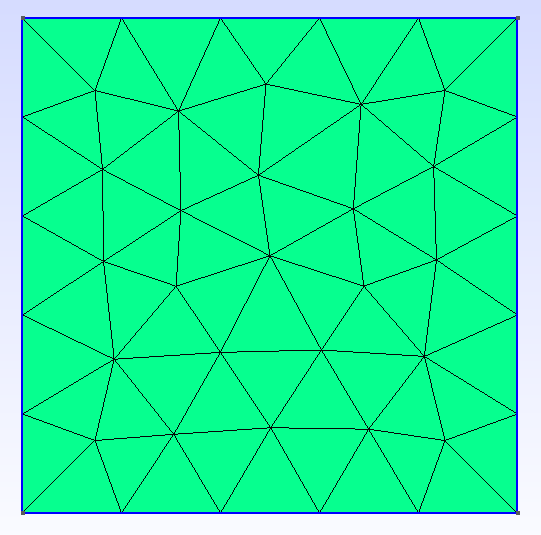
\includegraphics{figures/solid_angle_mesh.png}
    \caption{Solid Angle Mesh for $\theta\in[0,\pi/2]$, $\varphi\in[0,\pi/2]$}
  \end{figure}
  \framebreak

  \begin{figure}
    \begin{subfigure}{0.45\textwidth}
      \centering
      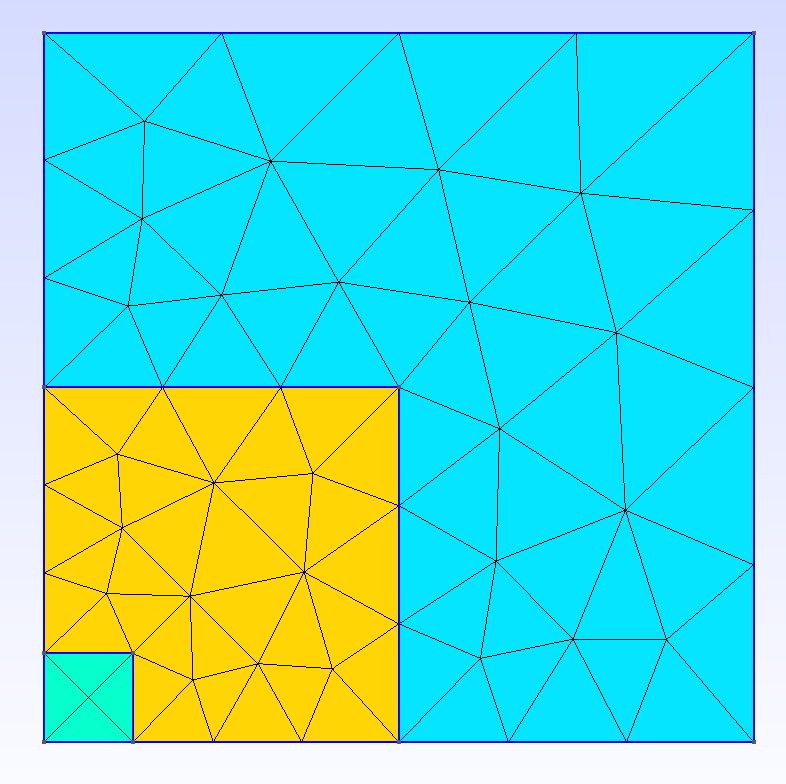
\includegraphics[width=0.65\textwidth]{figures/square_source/square_mesh_coarse.png}
      \subcaption{Coarse Mesh}
    \end{subfigure}%
    \begin{subfigure}{0.45\textwidth}
      \centering
      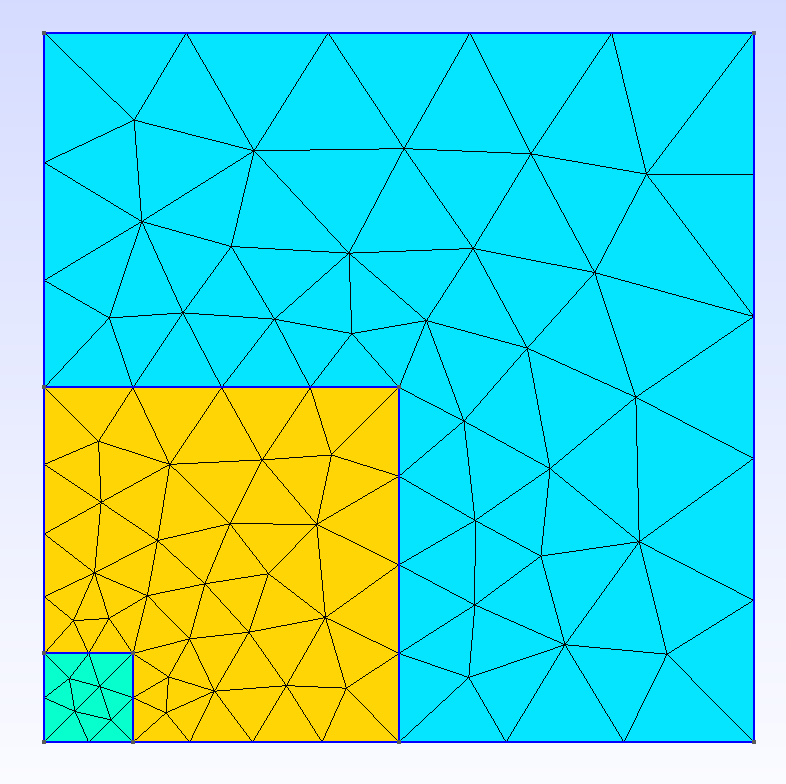
\includegraphics[width=0.65\textwidth]{figures/square_source/square_source_fine.png}
      \subcaption{Fine Mesh}
    \end{subfigure}
    \begin{subfigure}{0.45\textwidth}
      \centering
      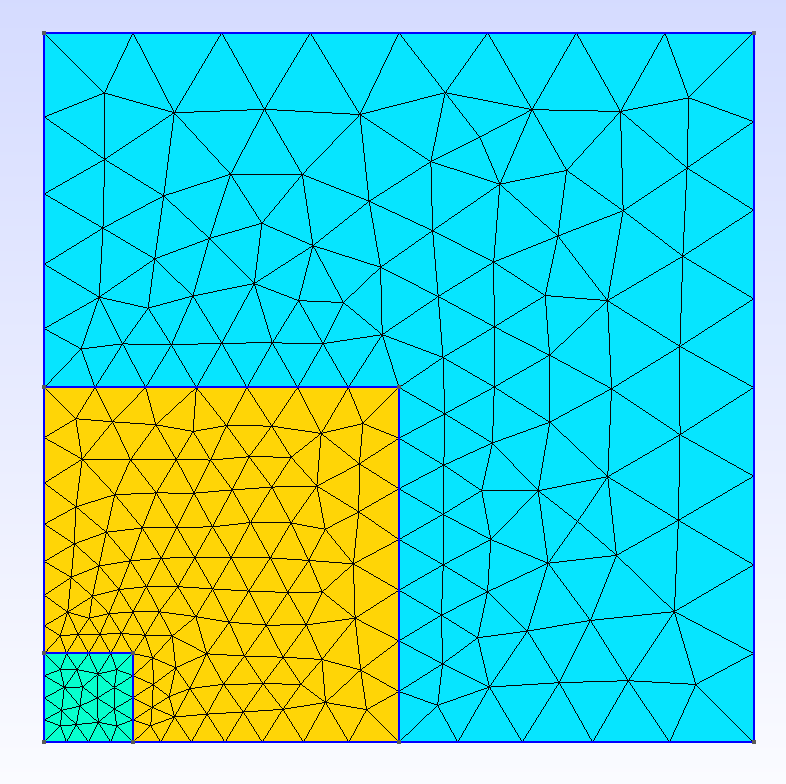
\includegraphics[width=0.65\textwidth]{figures/square_source/square_mesh_very_fine.png}
      \subcaption{Finer Mesh}
    \end{subfigure}%
  \end{figure}
\end{frame}
\framebreak

\begin{figure}
  \begin{subfigure}{0.45\textwidth}
    \centering
    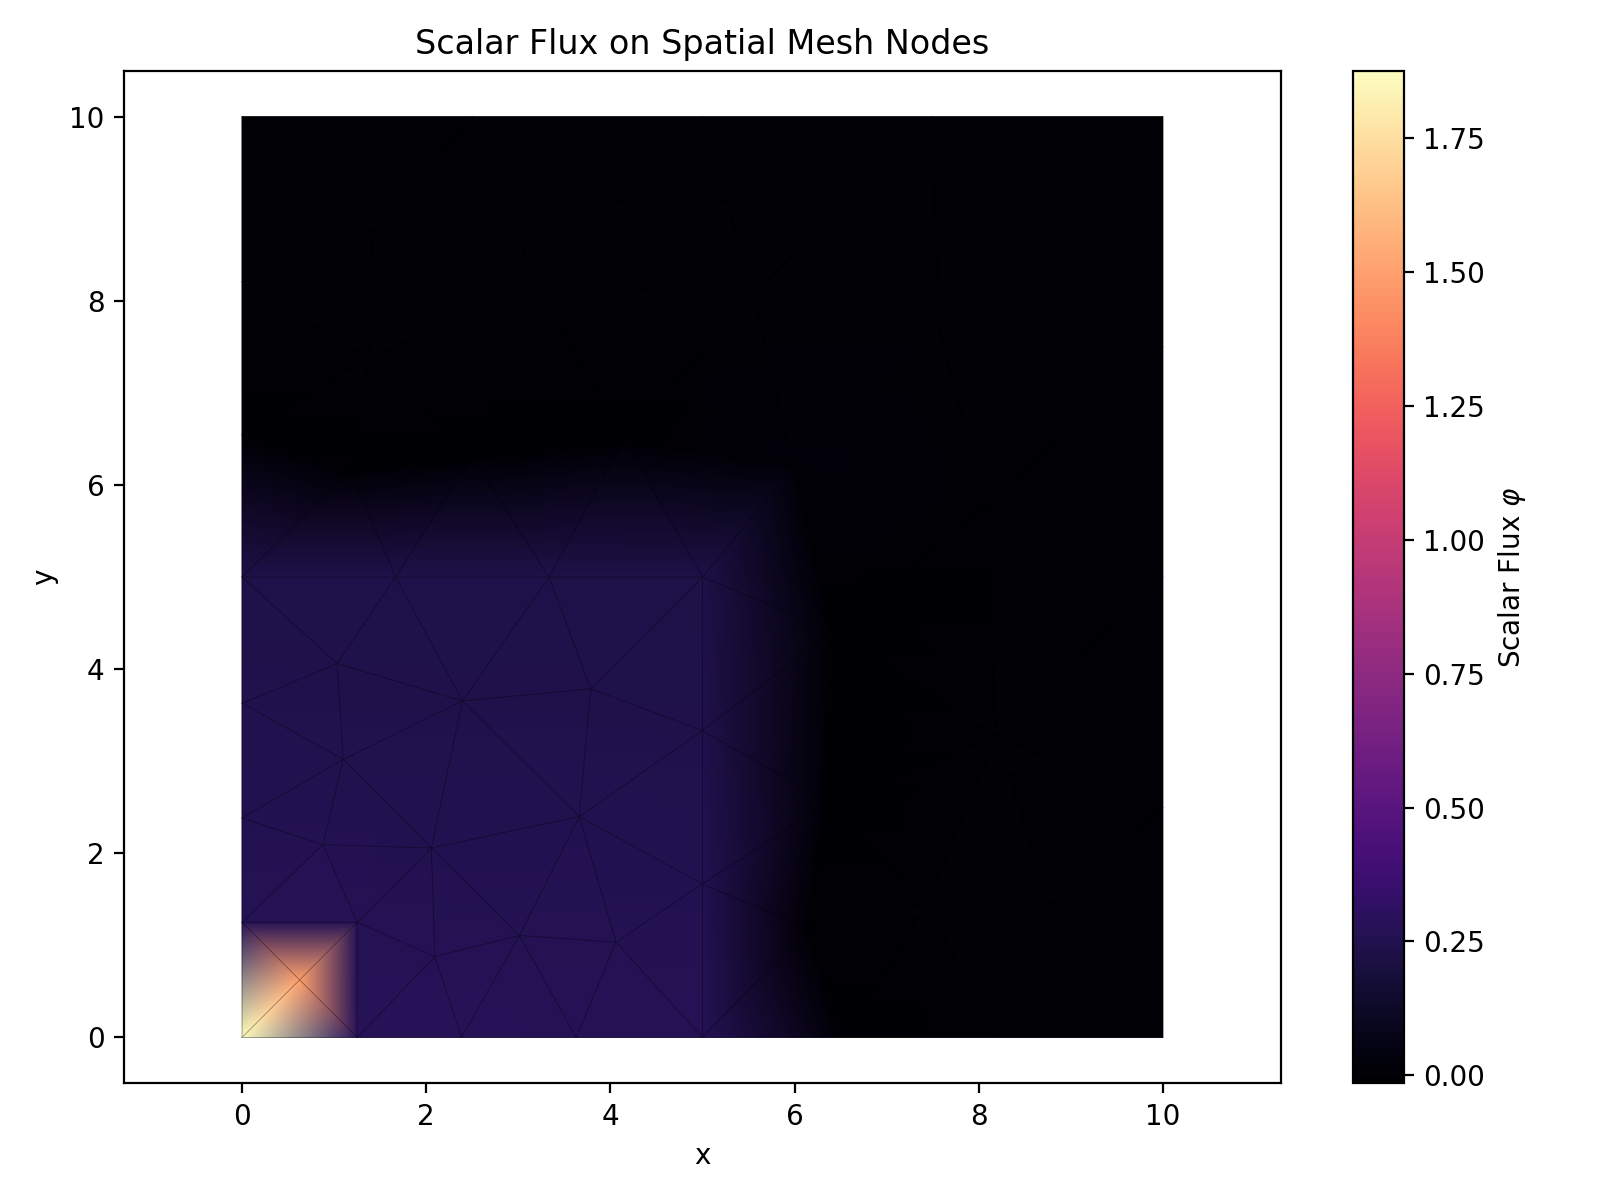
\includegraphics[width=0.65\textwidth]{figures/square_source/scalar_flux_coarse.png}
    \subcaption{Coarse Mesh}
  \end{subfigure}%
  \begin{subfigure}{0.45\textwidth}
    \centering
    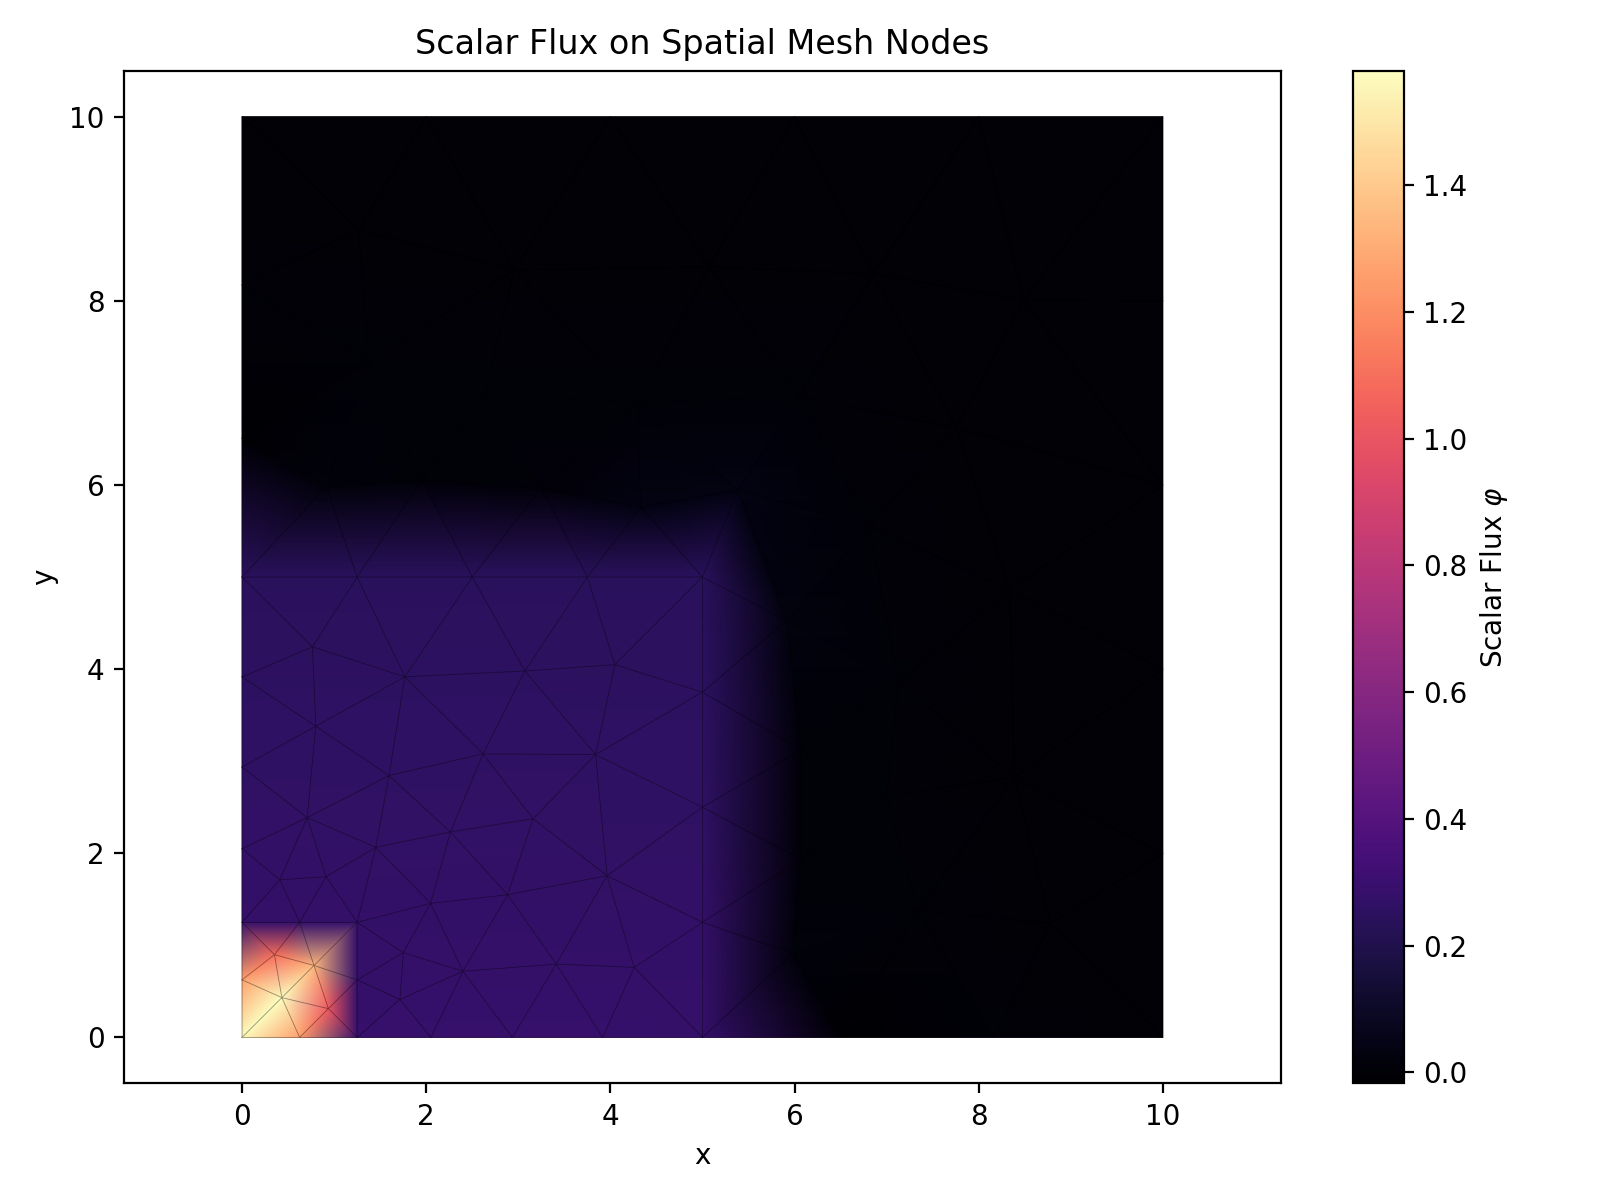
\includegraphics[width=0.65\textwidth]{figures/square_source/scalar_flux_fine.png}
    \subcaption{Fine Mesh}
  \end{subfigure}
  \begin{subfigure}{0.45\textwidth}
    \centering
    \includegraphics[width=0.65\textwidth]{figures/square_source/scalar_flux_finer.png}
    \subcaption{Finer Mesh}
  \end{subfigure}%
\end{figure}
\framebreak

\begin{figure}
  \begin{subfigure}{0.45\textwidth}
    \centering
    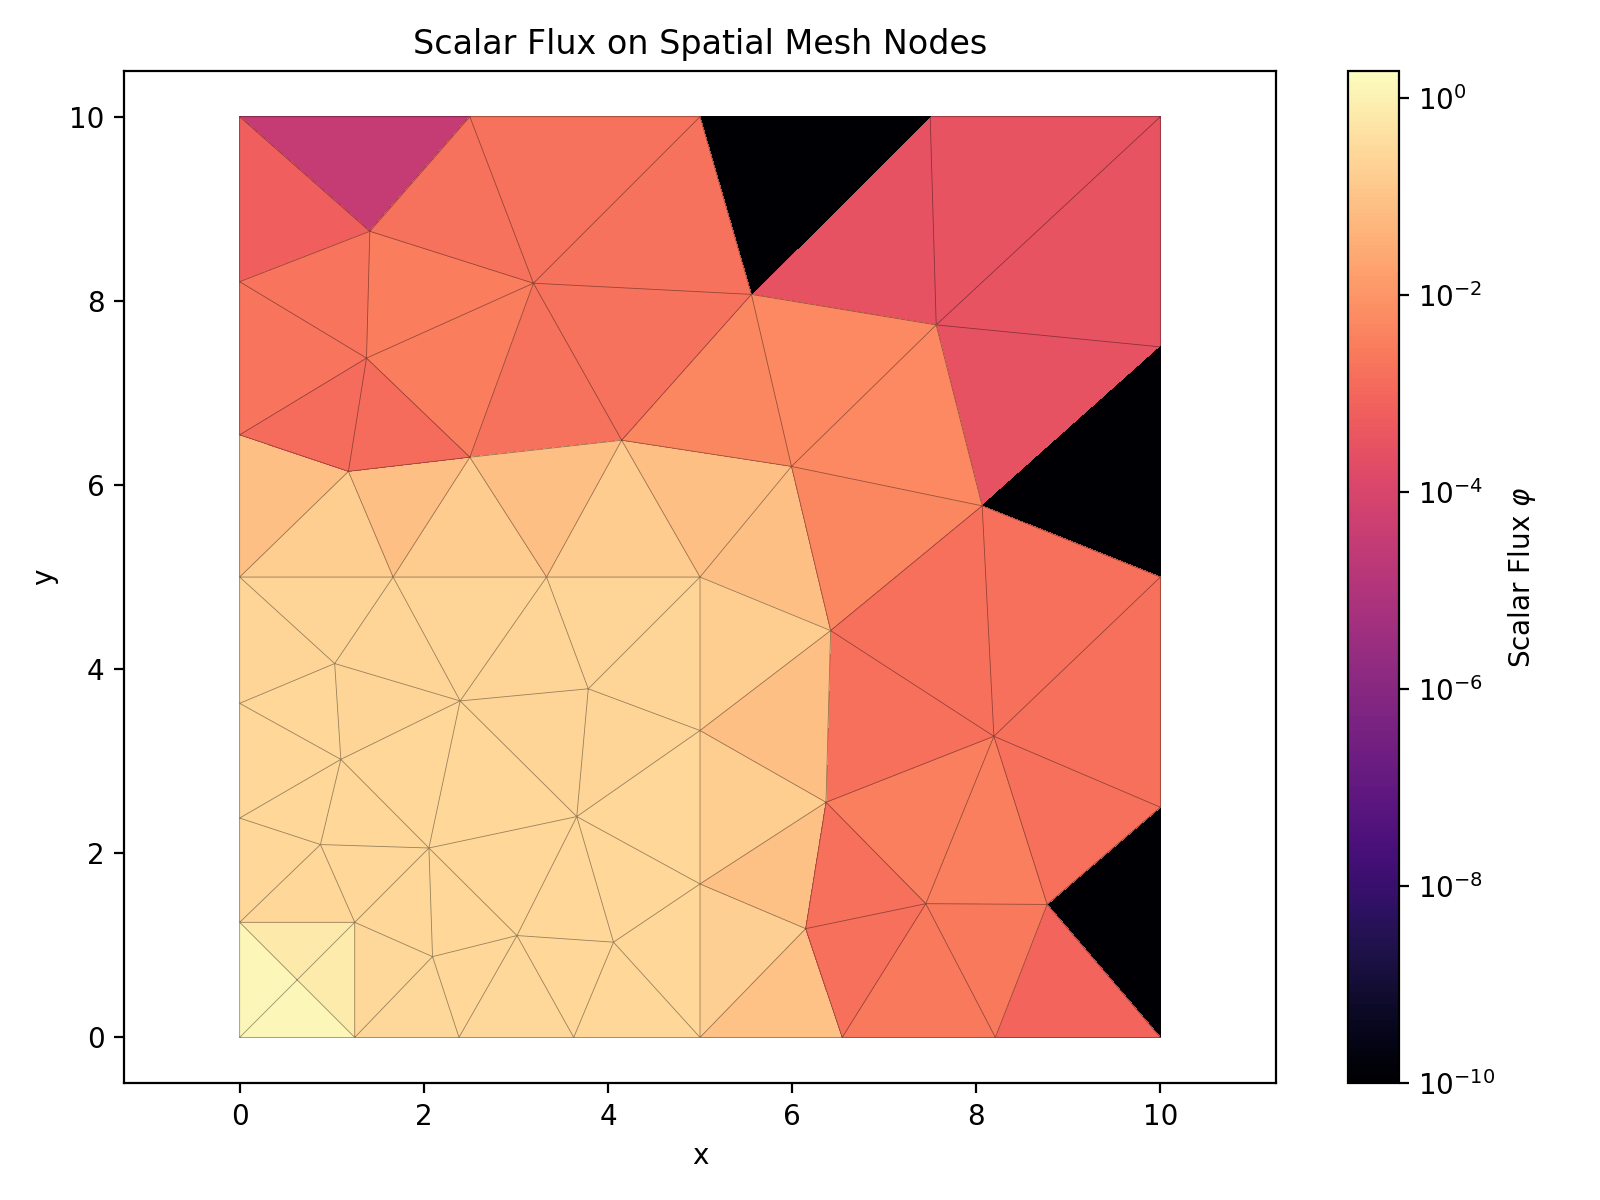
\includegraphics[width=0.65\textwidth]{figures/square_source/scalar_flux_log_coarse.png}
    \subcaption{Coarse Mesh}
  \end{subfigure}%
  \begin{subfigure}{0.45\textwidth}
    \centering
    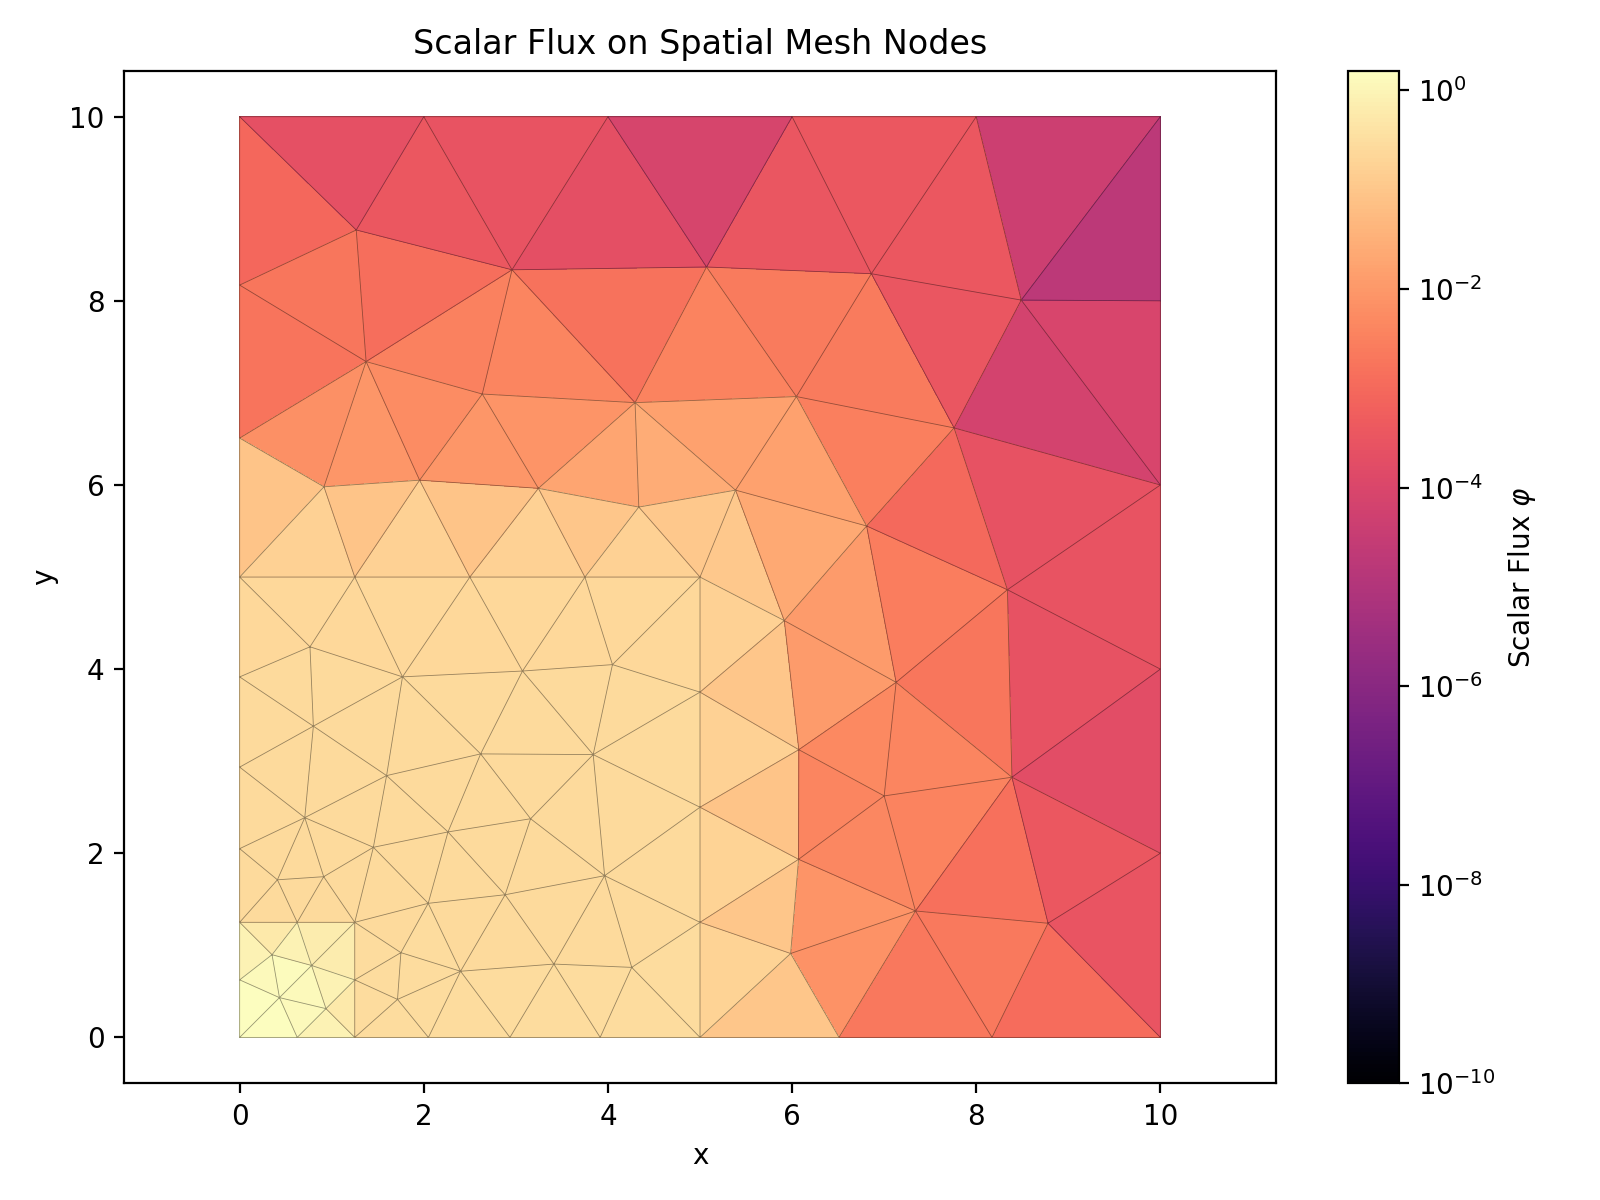
\includegraphics[width=0.65\textwidth]{figures/square_source/scalar_flux_log_fine.png}
    \subcaption{Fine Mesh}
  \end{subfigure}
  \begin{subfigure}{0.45\textwidth}
    \centering
    \includegraphics[width=0.65\textwidth]{figures/square_source/scalar_flux_log_finer.png}
    \subcaption{Finer Mesh}
  \end{subfigure}%
\end{figure}
\end{frame}

\section{Spherical Harmonics - Methods}
\input{spherical-harmonics.tex}

\section{Spherical Harmonics - Results}
\begin{frame}
  \frametitle{Problem Descriptions}
  The results slides will solve the same benchmarks with the same discretizations as the original discrete-ordinates methods to demonstrate the removal of the ray effect via spherical harmonics. \\

  As a reminder, the ray effect is the persistence of flux in the solvers sweeping directions, and is particularly apparent in geometries with low scattering.
\end{frame}

\begin{frame}
  \frametitle{\glspl{arp1} Absorbing Medium Results}
  \begin{figure}[b]
    \centering
    \begin{subfigure}{0.45\textwidth}
      \centering
      \includegraphics[width=0.65\textwidth]{figures/absorbing/cell_fluxes_256_8.png}
      \subcaption{$N=256$}
    \end{subfigure}%
    \begin{subfigure}{0.45\textwidth}
      \centering
      \includegraphics[width=0.65\textwidth]{figures/absorbing/cell_fluxes_1024_8.png}
      \subcaption{$N=1024$}
    \end{subfigure}
    \begin{subfigure}{0.45\textwidth}
      \centering
      \includegraphics[width=0.65\textwidth]{figures/absorbing/cell_fluxes_4096_8.png}
      \subcaption{$N=4096$}
    \end{subfigure}%
    \begin{subfigure}{0.45\textwidth}
      \centering
      \includegraphics[width=0.65\textwidth]{figures/absorbing/cell_fluxes_16384_8.png}
      \subcaption{$N=16384$}
    \end{subfigure}
    \caption{Solution of absorbing \glspl{arp1} for varying $N$ with $S_{8}$.}
  \end{figure}
\end{frame}


\section{Conclusion}
\begin{frame}
      \frametitle{Conclusions}
      % conclusions
      \begin{itemize}
            \item The even-odd-parity transformation is used to convert the hyperbolic \gls{bte} to an elliptic form while also reducing the angular computational domain to a quarter of the unit sphere.
            \item Both linear elements in angle and spherical harmonics expansions removes ray effects seen by the $S_N$ method.
            \item Linear angular methods may introduce additional diffusion of the solution, especially for localized sources, which may be undesirable.
            \item Computation time for spherical harmonics increases dramatically with an increase in order.
      \end{itemize}
\end{frame}



\section{Extra Slides}
\begin{frame}
  \frametitle{Legendre Polynomial Expansion of Inscattering Term}
  It is common to rewrite the inscattering (double-differential) cross section in terms of a Legendre polynomial expansion~\cite{Larsen2010}:
  \begin{equation}
    \label{eq:scattering-poly-expansion}
    \Sigma_s \left(\rvec,\ohat'\cdot \ohat,E'\rightarrow E\right) = \sum_{m=0}^{\infty}\frac{2m+1}{4\pi}P_m \left(\ohat' \cdot \ohat \right)\Sigma_{s,m}\left(\rvec, E'\rightarrow E\right)
  \end{equation}
  where $\Sigma_{s,m}\left(\rvec, E'\rightarrow E\right)$ are the \textit{Legendre moments}, computed with~\cite{TheoryManualOpenSn}:
  \begin{equation} \label{eq:legendre-moments}
    \Sigma_{s,m}\left(\rvec, E'\rightarrow E\right) = 2\pi \int_{-1}^{1}\Sigma_s \left(\rvec,\mu_0,E'\rightarrow E\right)P_m \left(\mu_0\right)\dd \mu_0
  \end{equation}
  where $\mu_0 \equiv \ohat' \cdot \ohat$.
  The moments are normally computed or available \textit{before} the simulation, \textit{not} computed on-the-fly.
  Note that \cref{eq:legendre-moments} is just an integral of the inscattering cross section over the unit sphere weighted by a Legendre polynomial.
\end{frame}

\begin{frame}
  \frametitle{Simplification of the \gls{bte}}
  Because the \glspl{arp} are stated to be \textit{non-multiplying}, \textit{time-independent}, and \textit{one-speed}, \cref{eq:general-bte} is immediately simplified to:
  \begin{multline}\label{eq:first-simplification-bte}
    \ohat \cdot \grad \psisimple + \Sigma_t \left(\rvec\right)\psisimple =\\=\int_{4\pi}\sum_{m=0}^{\infty}\frac{2m+1}{4\pi}P_m \left(\ohat' \cdot \ohat \right)\Sigma_{s,m}\left(\rvec\right)\psi \left(\rvec,\ohat'\right) \dd \ohat' + \frac{Q\left(\rvec\right)}{4\pi}
  \end{multline}
  Note that we have also substituted in \cref{eq:scattering-poly-expansion}.
\end{frame}

\begin{frame}
  \frametitle{Simplification of the \gls{bte}}
  The use of constant-value properties has a couple of immediate consequences, notably in the inscatter term.
  For a constant-value isotropic scattering cross section, \cref{eq:legendre-moments} is readily evaluated:
  \begin{equation}\label{eq:inscatter-xs-evaluated}
    \begin{split}
      \Sigma_{s,m}\left(\rvec\right) & = 2\pi \int_{-1}^{1}\Sigma_s \left(\rvec,\mu_0\right)P_m \left(\mu_0\right)\dd \mu_0       \\
                                     & =2\pi \int_{-1}^{1}\frac{\Sigma_s\left(\rvec\right)}{4\pi} P_m \left(\mu_0\right)\dd \mu_0 \\
                                     & =\frac{\Sigma_s\left(\rvec\right)}{2}\int_{-1}^{1} P_m \left(\mu_0\right)\dd \mu_0         \\
                                     & =\Sigma_s\left(\rvec\right) \delta_{0m}
    \end{split}
  \end{equation}
  where, in the last line, the orthogonality of Legendre polynomials is applied.

\end{frame}

\begin{frame}
  \frametitle{Simplification of the \gls{bte}}
  Substitution of \cref{eq:inscatter-xs-evaluated} into \cref{eq:first-simplification-bte} gives:
  \begin{equation}
    \ohat \cdot \grad \psisimple + \Sigma_t \left(\rvec\right)\psisimple =\frac{\Sigma_s\left(\rvec\right)}{4\pi}\int_{4\pi}\psi \left(\rvec,\ohat'\right) \dd \ohat' + \frac{Q\left(\rvec\right)}{4\pi}
  \end{equation}
  Or:
  \begin{equation} \label{eq:fully-simplified-bte-repeated}
    \ohat \cdot \grad \psisimple + \Sigma_t \left(\rvec\right)\psisimple =\frac{\Sigma_s\left(\rvec\right)}{4\pi}\phi\left(\rvec\right) + \frac{Q\left(\rvec\right)}{4\pi}
  \end{equation}
  where:
  \begin{equation}
    \label{eq:scalar-flux-repeated}
    \phi\left(\rvec\right)\equiv \int_{4\pi}\psi \left(\rvec,\ohat\right) \dd \ohat
  \end{equation}
  \Cref{eq:scalar-flux} is know as the \textit{angle-integrated} (or \textit{scalar}) \textit{flux}.
\end{frame}

\begin{frame}
  \frametitle{Error Plot}
  \begin{figure}
    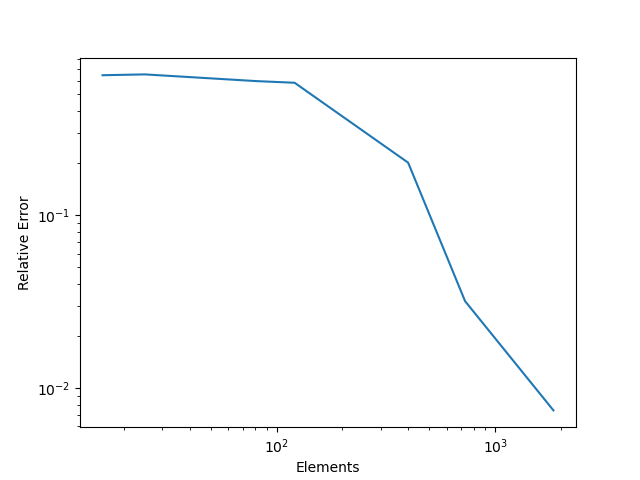
\includegraphics{figures/sphere/error.png}
    \caption{Error}
  \end{figure}
\end{frame}


% \input{acks}
%%--------------------------------%%
%%--------------------------------%%
\begin{frame}[allowframebreaks]
  \frametitle{References}
  \bibliographystyle{ieeetr}
  {\footnotesize \bibliography{bibliography.bib} }

\end{frame}

%%--------------------------------%%


\end{document}



